%----------------------------------------------------------------------------------------
%  CHAPTER CONTENTS
%----------------------------------------------------------------------------------------

\chapter*{Predicting gender in introductory CS}

\section*{Project Overview}

As I have often said, one of the biggest challenges of this century is successfully getting people into the technical workforce. We are now in the age of automation with autonomous cars driving down our streets and Alexa and Siri becoming an extension of our homes. With the increase of these systems, it is likely that we are also going to see an increase in technical jobs.

This shift in the workforce towards highly skilled, technical knowledge workers poses a challenge on the supply side; mostly because of a lack of presence of computer science in K-12 education; the under-production of post-secondary degrees in computer science;  the underrepresentation of women and the underrepresentation of ethnic minorities.

One of the solutions that have been proffered for this problems is redesigning introductory computer science to broadening participation.  

As part of my doctoral study, I decided to study the socio-curricular factors that affect the decision to participate in introductory computer science through a data-driven lens. To do this, I designed a research study investigating the role of computer science self-identity centered around the experiences of undergraduates in two introductory computer science classes at UC Berkeley.


\section*{Problem Statement}

With this project, the problem I am interested in investigating is the gendered experience of these the two CS classes in my study. Using machine learning algorithms, I want to predict and identify the most salient variables that govern the experience of men versus women in introductory CS at an elite research university like Berkeley.

To predict gender in intro CS at Berkeley we suggest the following strategy:
\begin{enumerate}% 
\item Explore the dataset to ensure its integrity and understand the context.
\item Identify features that may be used. If possible, engineer features that might provide greater discrimination.
\item With the understanding that this a ``classification'' task, explore a couple of classifiers that might be well suited for the problem at hand.
\item Once a classifier has been selected, tune it for optimality.
\end{enumerate}

\section*{Metrics}


Predicting gender in intro CS is a supervised learning problem. To determine the performance of the model, I have selected ``accuracy" as the metric of most interest. In addition to that, we will take a look at the confusion matrix for the output of each model to give us more insight into how good our classifiers are at discriminating the data based on gender. 

%----------------------------------------------------------------------------------------
%  CHAPTER 
%----------------------------------------------------------------------------------------

\chapter*{Analysis}

\section* {Dataset}
This project uses a dataset which I created as part of my doctoral research. The dataset consists of survey responses. A copy of the survey instrument can be found in the appendix of this report \ref{surveyInstrument}. The survey instruments were developed to measure participants' self-reported efficacy along several dimensions. 

\begin{enumerate}% 
\item Self-reported attitudes about CS
\item Gendered belief about CS ability
\item Career driven beliefs about CS
\item Self-reported attitudes about computational thinking
\item Self-reported attitudes about CS class belonging
\item Self-reported beliefs about collegiality
\item Prior collegiate CS exposure
\item CS mentors and role models
\end{enumerate}



Majority of the questionnaire uses a 5-point Likert scale (where 1 = Not Really, 3 = Neutral and 5 = Absolutely). The dataset consists of 882 instances with no missing data.



An interesting aspect of this dataset is that the class labels for our classification are slightly unbalanced at a ratio of around 1:1.2 for male students as can be seen in figure \ref{targetClass}. 

\begin{figure}[!hbtp]
\centering
    \subfloat[]{%
    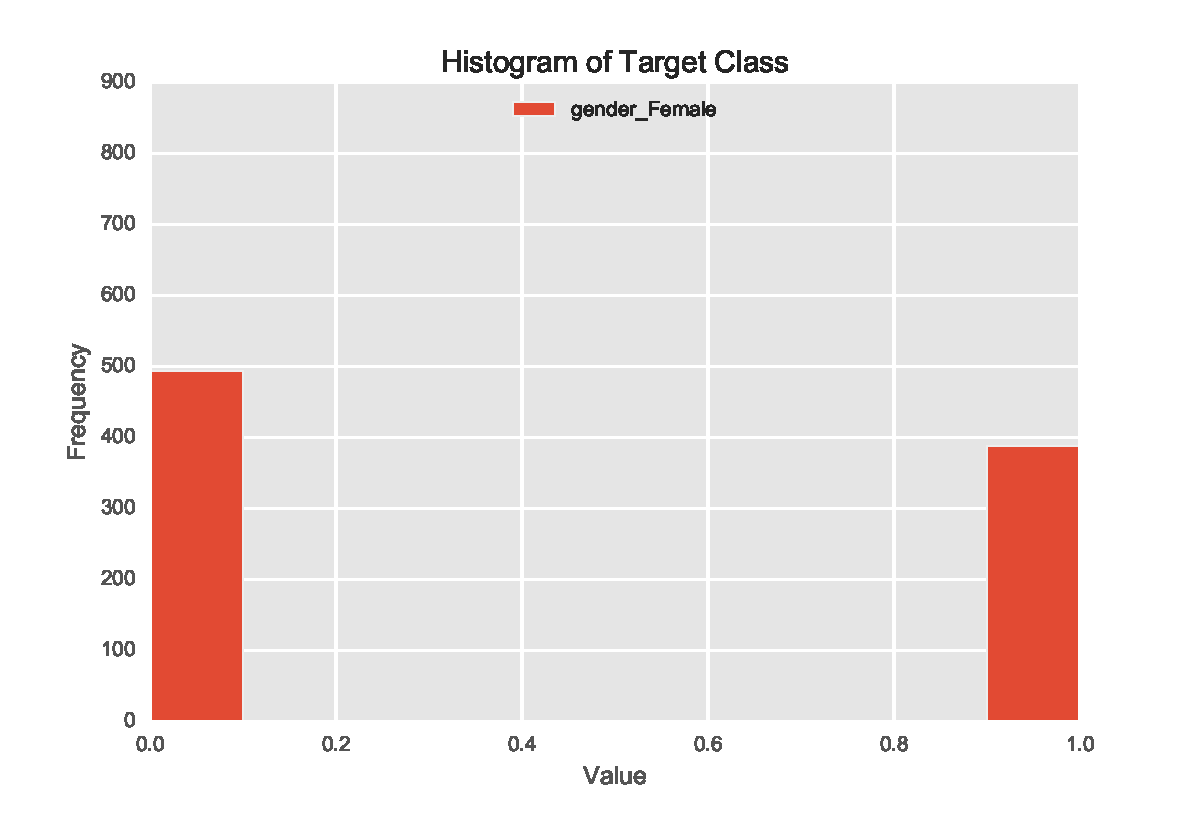
\includegraphics[width=0.8\textwidth]{figures/targetClass}
    \label{targetClass}}
    
    \caption{\textbf{Gender plot. }\textit{The histogram shows a slightly unbalanced target dataset with 494 values of \{0: male\} and 388 values of \{1: female\}.}}
\end{figure}



\section*{Algorithms and Techniques}

For the problem of predicting gender in intro CS I experimented with four different classifiers, a decision tree classifier, two ensemble methods and a support vector machine:

\begin{enumerate}% 
\item A RandomForestClassifier\\
I selected this learner because it is considered one of the best off-the-shelf learning algorithm, and requires almost no tuning. 
\item An eXtreme Gradient Boosted (XGBoost) Trees Classifier\\
XGBoost is an advanced implementation of gradient boosting algorithm. From reading literature on machine learning in practice, the XGBoost classifier has differentiated itself as a classifier that has successfully demonstrated its performance in a wide range of problems from particle physics, to ad click-through rate prediction and so on. For example, ``among the 29 challenge winning solutions published at Kaggle's blog during 2015, 17 solutions used XGBoost.''

\item Support Vector Machine (SVMs)\\
I selected the SVMs because they are very robust classifiers and \textit{more importantly}, they have a method of \textit{biasing} the soft-margin constant, $C$, to correct for class imbalances. 
              
\item Decision Tree Classifier\\
The \textit{major} reason why the decision tree classifier was selected was its interpretability. For this problem domain, it is not just satisfactory to discriminate between male and female students, what learning researchers ultimately want is to gain \textit{insights} into what the salient factors around the experience of intro CS are so they can correct for negative outcomes.

\end{enumerate}

\section*{Benchmark}

This is novel research, as a result, there are no benchmarks we can compare the performance of our classifiers with.


%----------------------------------------------------------------------------------------
%  CHAPTER 
%----------------------------------------------------------------------------------------
\chapter*{Methodology}


\section*{Data Preprocessing}

\subsection*{Preprocess feature columns}

To prepare our data for classification, we need to devise a scheme to transform all features into numeric data. This dataset as several non-numeric columns that need converting. Many of them are simply \texttt{yes} and \texttt{no}, e.g. \texttt{prcs\_2}. We can reasonably convert these into `1'/`0' (binary) values. For the columns whose values are `Nan', we will convert these to `0'.
\begin{itemize}% 
\item If the algorithms chosen require preprocessing steps like feature selection or feature transformations, have they been properly documented?
\item Based on the Data Exploration section, if there were abnormalities or characteristics that needed to be addressed, have they been properly corrected?
\item If no preprocessing is needed, has it been made clear why?
\end{itemize}

\section*{Implementation}
In this section, the process for which metrics, algorithms, and techniques that you implemented for the given data will need to be clearly documented. It should be abundantly clear how the implementation was carried out, and discussion should be made regarding any complications that occurred during this process. Questions to ask yourself when writing this section:
\begin{itemize}% 
\item Is it made clear how the algorithms and techniques were implemented with the given datasets or input data?
\item Were there any complications with the original metrics or techniques that required changing prior to acquiring a solution?
\item Was there any part of the coding process (e.g., writing complicated functions) that should be documented?
\end{itemize}


\section*{Refinement}
In this section, you will need to discuss the process of improvement you made upon the algorithms and techniques you used in your implementation. For example, adjusting parameters for certain models to acquire improved solutions would fall under the refinement category. Your initial and final solutions should be reported, as well as any significant intermediate results as necessary. Questions to ask yourself when writing this section:
\begin{itemize}% 
\item Has an initial solution been found and clearly reported?
\item Is the process of improvement clearly documented, such as what techniques were used?
\item Are intermediate and final solutions clearly reported as the process is improved?
\end{itemize}
%----------------------------------------------------------------------------------------
%  CHAPTER 
%----------------------------------------------------------------------------------------

\chapter*{Results}
(approximately 2 - 3 pages)


\section*{Model Evaluation and Validation}

When I did feature selection using SelectPercentile on top 10\% of the features, the model over-fitted, giving a 100\% score on all the three classifiers used.


In this section, the final model and any supporting qualities should be evaluated in detail. It should be clear how the final model was derived and why this model was chosen. In addition, some type of analysis should be used to validate the robustness of this model and its solution, such as manipulating the input data or environment to see how the model’s solution is affected (this is called sensitivity analysis). Questions to ask yourself when writing this section:
\begin{itemize}% 
\item Is the final model reasonable and aligning with solution expectations? Are the final parameters of the model appropriate?
\item Has the final model been tested with various inputs to evaluate whether the model generalizes well to unseen data?
\item Is the model robust enough for the problem? Do small perturbations (changes) in training data or the input space greatly affect the results?
\item Can results found from the model be trusted?
\end{itemize}

\section*{Justification}
In this section, your model’s final solution and its results should be compared to the benchmark you established earlier in the project using some type of statistical analysis. You should also justify whether these results and the solution are significant enough to have solved the problem posed in the project. Questions to ask yourself when writing this section:
\begin{itemize}% 
\item Are the final results found stronger than the benchmark result reported earlier?
\item Have you thoroughly analyzed and discussed the final solution?
\item Is the final solution significant enough to have solved the problem?
\end{itemize}

%----------------------------------------------------------------------------------------
%  CHAPTER 
%----------------------------------------------------------------------------------------

\chapter*{Conclusion}
(approximately 1 - 2 pages)

\section*{Free-Form Visualization}
In this section, you will need to provide some form of visualization that emphasizes an important quality about the project. It is much more free-form, but should reasonably support a significant result or characteristic about the problem that you want to discuss. Questions to ask yourself when writing this section:
\begin{itemize}% 
\item Have you visualized a relevant or important quality about the problem, dataset, input data, or results?
\item Is the visualization thoroughly analyzed and discussed?
\item If a plot is provided, are the axes, title, and datum clearly defined?
\end{itemize}


\section*{Reflection}
In this section, you will summarize the entire end-to-end problem solution and discuss one or two particular aspects of the project you found interesting or difficult. You are expected to reflect on the project as a whole to show that you have a firm understanding of the entire process employed in your work. Questions to ask yourself when writing this section:
\begin{itemize}% 
\item Have you thoroughly summarized the entire process you used for this project?
\item Were there any interesting aspects of the project?
\item Were there any difficult aspects of the project?
\item Does the final model and solution fit your expectations for the problem, and should it be used in a general setting to solve these types of problems?
\end{itemize}

\section*{Improvement}
In this section, you will need to provide discussion as to how one aspect of the implementation you designed could be improved. As an example, consider ways your implementation can be made more general, and what would need to be modified. You do not need to make this improvement, but the potential solutions resulting from these changes are considered and compared/contrasted to your current sLike Sita's family, mine where non-pleased with my choice. olution. Questions to ask yourself when writing this section:
\begin{itemize}% 
\item Are there further improvements that could be made on the algorithms or techniques you used in this project?
\item Were there algorithms or techniques you researched that you did not know how to implement, but would consider using if you knew how?
\item If you used your final solution as the new benchmark, do you think an even better solution exists?
\end{itemize}